\documentclass[11pt,a4paper]{article}
\usepackage[utf8]{inputenc}
\usepackage[dutch]{babel}
\usepackage{pgfplots}
\usepgfplotslibrary{units}
\usepackage{float}
\usepackage{amsmath,amsthm}
\usepackage{amsfonts}
\usepackage{amssymb,marvosym}
\usepackage[left=2cm,right=2cm,top=2.5cm,bottom=2cm]{geometry}
\usepackage{graphicx}
\usepackage{multicol}
\usepackage{enumerate}
\usepackage{fancyhdr}
\pagestyle{fancy}
\usepackage{algorithm}
\usepackage{algpseudocode}
\usepackage{pgfplots}
\usepackage{multirow}
\usepackage{tikz}
\usetikzlibrary{arrows}
\usetikzlibrary{calc}

\floatname{algorithm}{Algoritme}


\usepackage[font=small,labelfont=bf]{caption}
\captionsetup[table]{aboveskip=-0.8em}
\captionsetup[table]{belowskip=-0.7pt}


\lhead {Proj. DAII: Genetische algoritmen} 
\chead{BAZ(~ \thepage ~ )NGA} 
\rhead{Robbert Gurdeep Singh}


\cfoot{} % get rid of the page number 

\usepackage{hyperref}
\usepackage{chngcntr}
\counterwithin*{section}{part}
\counterwithin{algorithm}{section}
\counterwithin{table}{section}
\counterwithin{figure}{section}

\hypersetup{
    colorlinks=false,
    pdfborder={0 0 0},
}

\author{Robbert Gurdeep Singh}
\title{{Project Algoritmen en datastructuren III}\\ \Huge Gedistribueerde Genetische algoritmen}
%\date{}



\pgfplotsset{compat=1.8}


\newcommand{\drawGraph}[4]{
\begin{tikzpicture}
\begin{axis}[scale only axis, 
	%x-as	
    xmin=0,
	xlabel=#1,	
	%y-as
	ylabel=#2,
	ymin=0,
	%Style
	height=5em,width=.37\textwidth,
	enlargelimits=0.05,
	grid=major,	legend pos=south east
]
#3
\end{axis}
\end{tikzpicture}
}


\newcommand{\lxaxis}[3]{\begin{tikzpicture}
\begin{axis}[scale only axis, 
cycle list name=exotic,
    xmode=log,
    log ticks with fixed point,
	%x-as	
	xlabel=#2,	
	%y-as
	ylabel=#1,
	ymin=0,
	%Style
	height=5em,width=.37\textwidth,
	enlargelimits=0.05,
	grid=major,	legend pos=south east
]
#3

\end{axis}
\end{tikzpicture}}

\newcommand{\rlxaxis}[3]{\begin{tikzpicture}
\begin{axis}[scale only axis, 
cycle list name=exotic,
    xmode=log,
    log ticks with fixed point,
	%x-as	
	xlabel=#2,	
	%y-as
	ylabel=#1,
	%Style
	height=5em,width=.37\textwidth,
	enlargelimits=0.05,
	grid=major,	legend pos=south east
]
#3

\end{axis}
\end{tikzpicture}}

\newcommand{\nxaxis}[3]{\begin{tikzpicture}
\begin{axis}[scale only axis,
cycle list name=exotic, 
	%x-as	
    xmin=0,
	xlabel=#2,	
	%y-as
	ylabel=#1,
	ymin=0,
	%Style
	height=5em,width=.37\textwidth,
	enlargelimits=0.05,
	grid=major,	legend pos=south east
]
#3

\end{axis}
\end{tikzpicture}}


\newcommand{\nxaxisr}[3]{\begin{tikzpicture}
\begin{axis}[scale only axis,
cycle list name=exotic, 
	%x-as	
	xlabel=#2,	
	%y-as
	ylabel=#1,
	ymin=0,
	%Style
	height=5em,width=.37\textwidth,
	enlargelimits=0.05,
	grid=major,	legend pos=south east
]
#3

\end{axis}
\end{tikzpicture}}

\newcommand{\rnxaxis}[3]{\begin{tikzpicture}
\begin{axis}[scale only axis, 
cycle list name=exotic,
	%x-as	
    xmin=0,
	xlabel=#2,	
	%y-as
	ylabel=#1,
	%Style
	height=5em,width=.37\textwidth,
	enlargelimits=0.05,
	grid=major,	legend pos=south east
]
#3

\end{axis}
\end{tikzpicture}}


\newcommand{\rnxaxisr}[3]{\begin{tikzpicture}
\begin{axis}[scale only axis, 
cycle list name=exotic,
	%x-as	
	xlabel=#2,	
	%y-as
	ylabel=#1,
	%Style
	height=5em,width=.37\textwidth,
	enlargelimits=0.05,
	grid=major,	legend pos=south east
]
#3

\end{axis}
\end{tikzpicture}}


\newcommand{\itemMB}[1]{
	\item[$\boldsymbol{#1}$:]
}

\newcommand{\itembf}[1]{
	\item \textbf{#1}:
}



\newcommand{\abs}[1]{
	\lvert #1 \rvert
}

\newcommand{\addploti}[1]{\addplot table [y=i, x=testValue, col sep=comma] {../../tests/param_results/#1.log};}
\newcommand{\addplotf}[1]{\addplot table [y=f, x=testValue, col sep=comma] {../../tests/param_results/#1.log};}
\newcommand{\addplott}[1]{\addplot table [y=t, x=testValue, col sep=comma] {../../tests/param_results/#1.log};}

\definecolor{mymark}{HTML}{EBB8B8}

\begin{document}

\twocolumn[\begin{@twocolumnfalse}
    \maketitle
    
    \begin{abstract}
    	{\em
    	In dit verslag bespreken we de implementatie van een genetisch algoritmen. We onderzoeken wat de optimale parameters zijn en vergelijken enkele algoritmen.
    	}
    \end{abstract}
    
\end{@twocolumnfalse}]
% grep  '\s*\\label' * | sed "s/\s\s*/ /g;s/:/+/;s/\+ /+/;s/^/%/" | column -t -s+
%algoritmen_crossover.tex                      \label{sub:crossover}
%algoritmen_crossover.tex                      \label{alg:crossover-1point}
%algoritmen_crossover.tex                      \label{alg:crossover-random}
%algoritmen_inpoly.tex                         \label{sub:algo-pt-in-poly}
%algoritmen_inpoly.tex                         \label{alg:inPolygon}
%algoritmen_mutation.tex                       \label{sub:Mutation}
%algoritmen_mutation.tex                       \label{ssub:MutationAlgorithm}
%algoritmen_mutation.tex                       \label{alg:Mutation}
%algoritmen_mutation.tex                       \label{ssub:MutationImplementation}
%algoritmen_mutation.tex                       \label{ssub:MutationComplexity}
%algoritmen_stochastic_universal_sampling.tex  \label{sub:SUS}
%algoritmen_stochastic_universal_sampling.tex  \label{fig:SUS}
%algoritmen_stochastic_universal_sampling.tex  \label{alg:SUS}
%algoritmen_stochastic_universal_sampling.tex  \label{ssub:SUSComplexity}
%algoritmen.tex                                \label{sec:algoritmen}
%algoritmen_tournament.tex                     \label{sub:tournament}
%algoritmen_tournament.tex                     \label{alg:tournament}
%algoritmen_tournament.tex                     \label{ssub:notetournament}
%verslag.tex                                   \label{sec:inleiding}
%verslag.tex                                   \label{sec:explainationcode}
%verslag.tex                                   \label{sub:pointer}

\part{Genetisch algoritme}
\section{Inleiding}
\label{sec:inleiding}
Het probleem dat we trachten op te lossen is het volgende: %TODO
Als we het vanaf nu hebben over een veelhoek dan bedoelen we een convexe veelhoek.

\subsection{Gebruikte symbolen}
Tenzij anders vermeld betekenen volgende symbolen het volgende:
\begin{itemize}
\itemMB{n} Het aantal te plaatsen punten
\itemMB{X_i} Het i-de individu 
\itemMB{z} Het aantal zijden van de veelhoek
\itemMB{N_p} Populatiegrootte
\itemMB{P_M} Mutatiedruk 
\itemMB{f} De fitheidsfunctie \[f(X_k)= \sum_{P_1 \in X_k}\sum_{P_2 \in X_k} \sqrt{d_2(P_1,P_2)} \]
\end{itemize}

%\subsection{Overzicht}
%\tableofcontents

% subsection  (end)
% section inleiding (end)

\section{Algortitmen}
\subsection{Punt in veelhoek}
\label{sub:algo-pt-in-poly}
Eén van de voorwaarden waaraan een oplossing moet voldoen is dat alle punten \textbf{in} de veelhoek liggen.Het is dus noodzakelijk om een algoritme te hebben dat bepaalt of een punt zich al dan niet in de convexe veelhoek bevind.
\subsubsection{Idee}
Trekken we een lijn vanuit het punt ``naar boven'', dan kunnen we 3 gevallen onderscheiden:
\begin{itemize}
\item We snijden de veelhoek niet ($P_{1}$): \\
		We weten dat we ons niet binnen de veelhoek bevonden.
\item We snijden de veelhoek juist 1 keer ($P_{2}$):\\
		Nu zijn we zeker in de veelhoek. 
\item We snijden de veelhoek juist\footnote{Merk op dat indien we de veelhoek meer dan 2 keer snijden, we kunnen aantonen dat de veelhoek niet convex is.} 2 keer ($P_{3}$):\\
		We liggen onder en dus ook buiten de veelhoek.
\end{itemize}

\begin{center}
\begin{figure}[H]
\centering
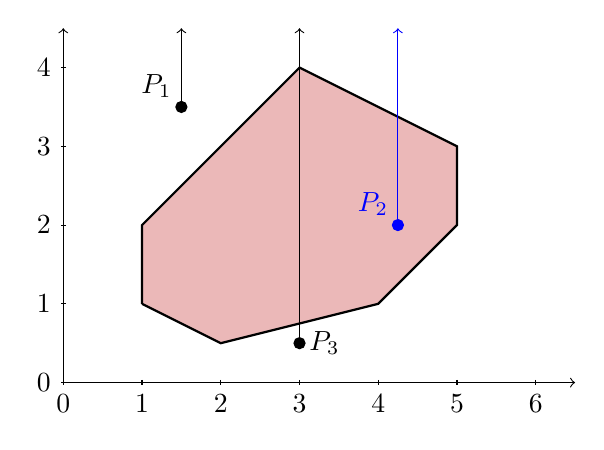
\begin{tikzpicture}
\draw[->] (0,0) -- (6.5,0);
\draw[->] (0,0) -- (0,4.5);

\foreach \x in {0,1,2,3,4,5,6}
    \draw (\x cm,1pt) -- (\x cm,-1pt) node[anchor=north] {\x};
\foreach \y in {0,1,2,3,4}
    \draw (1pt,\y cm) -- (-1pt,\y cm) node[anchor=east] {\y};

\draw[thick,fill=mymark] 
      (1,1) -- (1,2) -- 
	  (3,4) -- (5,3) -- 
	  (5,2) -- (4,1) -- 
	  (2,0.5) -- (1,1);
	  
	  
\coordinate (out1)    at (1.5,3.5);
\coordinate (out1top) at (1.5,4.5);
\filldraw[black] (out1) circle (2pt) node[anchor=south east] {$P_{1}$};

\coordinate (out2)    at (4.25,2);
\coordinate (out2top) at (4.25,4.5);
\filldraw[blue] (out2) circle (2pt) node[anchor=south east] {$P_{2}$};

\coordinate (out3)    at (3,0.5);
\coordinate (out3top) at (3,4.5);
\filldraw[black] (out3) circle (2pt) node[anchor=west] {$P_{3}$};


\draw[->] (out1) -- (out1top);
\draw[->,blue] (out2) -- (out2top);
\draw[->] (out3) -- (out3top);
\end{tikzpicture}
\caption{Punten binnen en buiten de figuur \texttt{soos.poly} met snijpunten.}
\end{figure}
\end{center}
We moeten dus nagaan dat een lijn ``naar boven'' vanuit het punt de veelhoek
juist één keer snijd.


\subsubsection{Algoritme}
Om te tellen hoe vaak we de veelhoek snijden, gaan we als volgt te werk:
Bij het inlezen van de veelhoek stellen we vergelijkingen op van de zijden van de 
veelhoek. Deze zijn van de vorm $y=a \cdot x+b$. Met $a = \infty$ als de rechte evenwijdig is met de $y$-as. 



	\begin{algorithm}[H]
	 	\caption{Bepalen of een punt in een veelhoek ligt}
		\begin{algorithmic}
		\Require zijden, een lijst van de zijden van een convexe veelhoek.
		%\Ensure T is gebalanceerd
		\Function{inPolygon}{$P_x$,$P_y$}
		\State count $\gets$ 0
		
		\For{\textbf{each} z $\in$ zijden} 
		\State $(x_1,y_1)$ $\gets$ $1^{ste}$ gedefinieerde punt van z
		\State $(x_2,y_2)$ $\gets$ $2^{de}$ gedefinieerde punt van z
		\If{z.$a = \infty \wedge x_1 = P_x$} 	\Comment z $\parallel$ $y$-as 
			\If{$P_y \in  \left \lbrack y_1,y_2\right\lbrack$}
			\State \Return \texttt{true} \Comment{Op lijn}
			\ElsIf{$y_1 > P_y$}
				\State count $\gets$ count$+1$
			\EndIf
		\Else	\Comment z $\not \parallel$ $y$-as
			\State $y_{inter}  \gets$ z.$a\cdot P_x +$z.$b$
			\If{$P_x \in  \left \lbrack x_1,x_2\right\lbrack$}
			
			\If{ $y_{inter} = P_y$ } 
				\State \Return \texttt{true} \Comment{Op lijn}
			\ElsIf{ $y_{inter} > P_y $} 
				\State count $\gets$ count$+1$
			\EndIf
				
			\EndIf
		\EndIf	

		\EndFor		

		\Return count == 1 ? \texttt{true} : \texttt{false}
		\EndFunction
		\end{algorithmic}
		\label{alg:inPolygon}
	\end{algorithm}		

Waarbij z$.a$ en z$.b$ de cooificienten zijn van de vergelijking $y=ax+b$ die de zijde 
voorstelt. De notatie van de intervallen houden geen rekening met de verhouding van de waarden ten opzichte van elkaar, wij bedoelen steeds de waarden tussen de gegeven waarden in of exclusief de grenzen.

\subsubsection{Complexiteit}
Kijken we naar algoritme \ref{alg:inPolygon} dan is het duidelijk dat de complexiteit $O(z)$ is met $z$ het aantal zijden.

% subsection  (end)

\subsubsection{Implementatie}
Deze methode is geimplementeerd in \\ \texttt{polygon.c} als  \texttt{polygon\_contains()}. 
We wijzen nog even op enkele details:
\begin{itemize}
\item We gebruiken $(P_x-x_1)\cdot(P_x-x_2)\leq0$ om te bepalen of een waarde al dan niet 
		tussen 2 waarden ligt. We doen dit zo omdat we niet weten hoe $x_1$ en $x_2$ 
		zich onderling verhouden.
\item Om het herberekenen van $a$ en $b$ te vermijden, berekenen we deze eenmalig bij het inlezen van de veelhoek.
\end{itemize}

\subsubsection{Genereren random punten}
\label{ssub:rand_generation}
Om random individuen voor de populatie te creëren genereren we telkens een random $x$ en $y$ binnen het omsloten vierkant. Vervolgens gaan we na of het ook wel degelijk in de veelhoek ligt. Telkens zo'n punt is gevonden wordt het toegevoegd aan het te genereren random individu tot er $n$ punten zijn. Voor het genereren van $N_p$ individuen heeft dit een complexiteit van $T(n)=\Theta(N_p\cdot n) = \Theta(n)$

% subsection  (end)

 

%\documentclass[11pt,a4paper]{article}
\usepackage[utf8]{inputenc}
\usepackage[dutch]{babel}
\usepackage{pgfplots}
\usepgfplotslibrary{units}
\usepackage{float}
\usepackage{amsmath,amsthm}
\usepackage{amsfonts}
\usepackage{amssymb,marvosym}
\usepackage[left=2cm,right=2cm,top=2.5cm,bottom=2cm]{geometry}
\usepackage{graphicx}
\usepackage{multicol}
\usepackage{enumerate}
\usepackage{fancyhdr}
\pagestyle{fancy}
\usepackage{algorithm}
\usepackage{algpseudocode}
\usepackage{pgfplots}
\usepackage{multirow}
\usepackage{tikz}
\usetikzlibrary{arrows}
\usetikzlibrary{calc}

\floatname{algorithm}{Algoritme}


\usepackage[font=small,labelfont=bf]{caption}
\captionsetup[table]{aboveskip=-0.8em}
\captionsetup[table]{belowskip=-0.7pt}


\lhead {Proj. DAII: Genetische algoritmen} 
\chead{BAZ(~ \thepage ~ )NGA} 
\rhead{Robbert Gurdeep Singh}


\cfoot{} % get rid of the page number 

\usepackage{hyperref}
\usepackage{chngcntr}
\counterwithin*{section}{part}
\counterwithin{algorithm}{section}
\counterwithin{table}{section}
\counterwithin{figure}{section}

\hypersetup{
    colorlinks=false,
    pdfborder={0 0 0},
}

\author{Robbert Gurdeep Singh}
\title{{Project Algoritmen en datastructuren III}\\ \Huge Gedistribueerde Genetische algoritmen}
%\date{}



\pgfplotsset{compat=1.8}


\newcommand{\drawGraph}[4]{
\begin{tikzpicture}
\begin{axis}[scale only axis, 
	%x-as	
    xmin=0,
	xlabel=#1,	
	%y-as
	ylabel=#2,
	ymin=0,
	%Style
	height=5em,width=.37\textwidth,
	enlargelimits=0.05,
	grid=major,	legend pos=south east
]
#3
\end{axis}
\end{tikzpicture}
}


\newcommand{\lxaxis}[3]{\begin{tikzpicture}
\begin{axis}[scale only axis, 
cycle list name=exotic,
    xmode=log,
    log ticks with fixed point,
	%x-as	
	xlabel=#2,	
	%y-as
	ylabel=#1,
	ymin=0,
	%Style
	height=5em,width=.37\textwidth,
	enlargelimits=0.05,
	grid=major,	legend pos=south east
]
#3

\end{axis}
\end{tikzpicture}}

\newcommand{\rlxaxis}[3]{\begin{tikzpicture}
\begin{axis}[scale only axis, 
cycle list name=exotic,
    xmode=log,
    log ticks with fixed point,
	%x-as	
	xlabel=#2,	
	%y-as
	ylabel=#1,
	%Style
	height=5em,width=.37\textwidth,
	enlargelimits=0.05,
	grid=major,	legend pos=south east
]
#3

\end{axis}
\end{tikzpicture}}

\newcommand{\nxaxis}[3]{\begin{tikzpicture}
\begin{axis}[scale only axis,
cycle list name=exotic, 
	%x-as	
    xmin=0,
	xlabel=#2,	
	%y-as
	ylabel=#1,
	ymin=0,
	%Style
	height=5em,width=.37\textwidth,
	enlargelimits=0.05,
	grid=major,	legend pos=south east
]
#3

\end{axis}
\end{tikzpicture}}


\newcommand{\nxaxisr}[3]{\begin{tikzpicture}
\begin{axis}[scale only axis,
cycle list name=exotic, 
	%x-as	
	xlabel=#2,	
	%y-as
	ylabel=#1,
	ymin=0,
	%Style
	height=5em,width=.37\textwidth,
	enlargelimits=0.05,
	grid=major,	legend pos=south east
]
#3

\end{axis}
\end{tikzpicture}}

\newcommand{\rnxaxis}[3]{\begin{tikzpicture}
\begin{axis}[scale only axis, 
cycle list name=exotic,
	%x-as	
    xmin=0,
	xlabel=#2,	
	%y-as
	ylabel=#1,
	%Style
	height=5em,width=.37\textwidth,
	enlargelimits=0.05,
	grid=major,	legend pos=south east
]
#3

\end{axis}
\end{tikzpicture}}


\newcommand{\rnxaxisr}[3]{\begin{tikzpicture}
\begin{axis}[scale only axis, 
cycle list name=exotic,
	%x-as	
	xlabel=#2,	
	%y-as
	ylabel=#1,
	%Style
	height=5em,width=.37\textwidth,
	enlargelimits=0.05,
	grid=major,	legend pos=south east
]
#3

\end{axis}
\end{tikzpicture}}


\newcommand{\itemMB}[1]{
	\item[$\boldsymbol{#1}$:]
}

\newcommand{\itembf}[1]{
	\item \textbf{#1}:
}



\newcommand{\abs}[1]{
	\lvert #1 \rvert
}

\newcommand{\addploti}[1]{\addplot table [y=i, x=testValue, col sep=comma] {../../tests/param_results/#1.log};}
\newcommand{\addplotf}[1]{\addplot table [y=f, x=testValue, col sep=comma] {../../tests/param_results/#1.log};}
\newcommand{\addplott}[1]{\addplot table [y=t, x=testValue, col sep=comma] {../../tests/param_results/#1.log};}

\definecolor{mymark}{HTML}{EBB8B8}

\begin{document}

\twocolumn[\begin{@twocolumnfalse}
    \maketitle
    
    \begin{abstract}
    	{\em
    	In dit verslag bespreken we de implementatie van een genetisch algoritmen. We onderzoeken wat de optimale parameters zijn en vergelijken enkele algoritmen.
    	}
    \end{abstract}
    
\end{@twocolumnfalse}]
\subsection{Tournament Selection}
\label{sub:tournament}
Tijdens de uitvoering van het genetisch algoritme zullen er steeds meer individuen bijkomen. We willen er echter voor zorgen dat onze populatie een vaste grootte ($N_p$) behoud. Er zullen dus individuen vermoord\footnote{Dat is dus verwijderden uit de populatie} moeten worden.
\subsubsection{Algoritme}
Om te bepalen we we vermoorden gebruiken we ``tournament selection''. Bij deze selectie word er telkens een vast aantal arbitraire individuen gekozen. Het individu met de slechtste fitheid uit deze groep wordt vervolgens vermoord. Dit wordt herhaald tot de populatie terug de juiste grootte heeft.
	\begin{algorithm}[H]
	 	\caption{Tournament-Select}
		\begin{algorithmic}
		\Require 
			\State $P$, te grote lijst van individuën 
			\State $N_p$, gewenste populatiegrootte
			\State $P_M$, de selectiedruk
		\Ensure returnt de index van verliezer
		\Function{tournamentSelection}{$P$,$N_t$}
		\State loser $\gets$ arbitraire waarde uit $\lbrace 0, \dots, \abs{P} \rbrace$

		\For{z $= 2 \rightarrow N_t$ } 
		\State j $\gets$ arbitraire waarde uit $\lbrace 0, \dots, \abs{P} \rbrace$
		\If{$f(X_j) < f(X_i)$}
			\State $loser \gets j$
		\EndIf
		\EndFor		
		\State \Return $loser$
		\EndFunction
		\\
		\\
		\While{$\abs{P} >  N_p$}
			\State $N_t \gets \left\lfloor\frac{P_M}{100} \cdot \abs{P}\right\rfloor$ 
			\State slachtoffer $\gets$ \Call{tournamentSelect}{$P$,$N_t$}
			\State $P \gets P\setminus$slachtoffer
		\EndWhile
		
		\end{algorithmic}
		\label{alg:tournament}
	\end{algorithm}		
\subsubsection{Complexiteit}
In algoritme \ref{alg:tournament} wordt er $\abs{P}-N_p$ keer een slachtoffer gekozen door een toernooi uit te voeren. Tijdens een toernooi wordt er $N_t$ keer een willekeurig individu gekozen en vergeleken. De complexiteit is dus $\Theta((\abs{P}-N_p)\cdot N_t)$. Met $N_t$ de toernooigrootte\footnote{Zie sectie \ref{sub:selection_pressure}} en $N_p$ de gewenste populatiegrootte. We zien dat $N_t$ hier gelijk is aan
 $\left\lfloor\frac{P_M}{100} \cdot \abs{P}\right\rfloor$.
 We bekomen dus: \[\Theta\left(\left(\abs{P}-N_p\right)\cdot P_m \cdot \abs{P}\right)\]
 Nu merken we op dat dit allemaal constanten\footnote{Enkel aanpasbaar bij compilatie} zijn binnen ons programma dus hebben we dat de complexiteit $T(n) = \Theta(1)$. 

% subsection  (end)

\subsubsection{Opmerking}
\label{ssub:notetournament}
Onder de aanvaarde aanname dat er minstens twee verschillende arbitraire indexen worden gekozen kunnen we stellen dat het beste individu steeds in de populatie blijft.
\begin{proof}
Stel dat het beste individu door tournament selection geselecteerd wordt om te vermoorden. Dan betekent dit dat hij een slechtere fitheid heeft dan de andere geselecteerden. Waaruit volgt dat hij niet het beste individu was.  \Lightning
\end{proof}
% subsubsection  (end)

\subsubsection{Implementatie}
Het bestand \texttt{genetic\_base.c} bevat de implementatie van Algoritme \ref{alg:tournament} in de functies \begin{itemize}
  \setlength{\itemsep}{1pt}
  \setlength{\parskip}{0pt}
  \setlength{\parsep}{0pt}
\item\texttt{do\_deathmatch()} en
\item\texttt{do\_neg\_tournament()}.
 \end{itemize}  


%\section{Bronnen}
Er moet vermeld worden dat het icosagon bestand afkomstig is van Jonathan Peck. 

\end{document}
%\documentclass[11pt,a4paper]{article}
\usepackage[utf8]{inputenc}
\usepackage[dutch]{babel}
\usepackage{pgfplots}
\usepgfplotslibrary{units}
\usepackage{float}
\usepackage{amsmath,amsthm}
\usepackage{amsfonts}
\usepackage{amssymb,marvosym}
\usepackage[left=2cm,right=2cm,top=2.5cm,bottom=2cm]{geometry}
\usepackage{graphicx}
\usepackage{multicol}
\usepackage{enumerate}
\usepackage{fancyhdr}
\pagestyle{fancy}
\usepackage{algorithm}
\usepackage{algpseudocode}
\usepackage{pgfplots}
\usepackage{multirow}
\usepackage{tikz}
\usetikzlibrary{arrows}
\usetikzlibrary{calc}

\floatname{algorithm}{Algoritme}


\usepackage[font=small,labelfont=bf]{caption}
\captionsetup[table]{aboveskip=-0.8em}
\captionsetup[table]{belowskip=-0.7pt}


\lhead {Proj. DAII: Genetische algoritmen} 
\chead{BAZ(~ \thepage ~ )NGA} 
\rhead{Robbert Gurdeep Singh}


\cfoot{} % get rid of the page number 

\usepackage{hyperref}
\usepackage{chngcntr}
\counterwithin*{section}{part}
\counterwithin{algorithm}{section}
\counterwithin{table}{section}
\counterwithin{figure}{section}

\hypersetup{
    colorlinks=false,
    pdfborder={0 0 0},
}

\author{Robbert Gurdeep Singh}
\title{{Project Algoritmen en datastructuren III}\\ \Huge Gedistribueerde Genetische algoritmen}
%\date{}



\pgfplotsset{compat=1.8}


\newcommand{\drawGraph}[4]{
\begin{tikzpicture}
\begin{axis}[scale only axis, 
	%x-as	
    xmin=0,
	xlabel=#1,	
	%y-as
	ylabel=#2,
	ymin=0,
	%Style
	height=5em,width=.37\textwidth,
	enlargelimits=0.05,
	grid=major,	legend pos=south east
]
#3
\end{axis}
\end{tikzpicture}
}


\newcommand{\lxaxis}[3]{\begin{tikzpicture}
\begin{axis}[scale only axis, 
cycle list name=exotic,
    xmode=log,
    log ticks with fixed point,
	%x-as	
	xlabel=#2,	
	%y-as
	ylabel=#1,
	ymin=0,
	%Style
	height=5em,width=.37\textwidth,
	enlargelimits=0.05,
	grid=major,	legend pos=south east
]
#3

\end{axis}
\end{tikzpicture}}

\newcommand{\rlxaxis}[3]{\begin{tikzpicture}
\begin{axis}[scale only axis, 
cycle list name=exotic,
    xmode=log,
    log ticks with fixed point,
	%x-as	
	xlabel=#2,	
	%y-as
	ylabel=#1,
	%Style
	height=5em,width=.37\textwidth,
	enlargelimits=0.05,
	grid=major,	legend pos=south east
]
#3

\end{axis}
\end{tikzpicture}}

\newcommand{\nxaxis}[3]{\begin{tikzpicture}
\begin{axis}[scale only axis,
cycle list name=exotic, 
	%x-as	
    xmin=0,
	xlabel=#2,	
	%y-as
	ylabel=#1,
	ymin=0,
	%Style
	height=5em,width=.37\textwidth,
	enlargelimits=0.05,
	grid=major,	legend pos=south east
]
#3

\end{axis}
\end{tikzpicture}}


\newcommand{\nxaxisr}[3]{\begin{tikzpicture}
\begin{axis}[scale only axis,
cycle list name=exotic, 
	%x-as	
	xlabel=#2,	
	%y-as
	ylabel=#1,
	ymin=0,
	%Style
	height=5em,width=.37\textwidth,
	enlargelimits=0.05,
	grid=major,	legend pos=south east
]
#3

\end{axis}
\end{tikzpicture}}

\newcommand{\rnxaxis}[3]{\begin{tikzpicture}
\begin{axis}[scale only axis, 
cycle list name=exotic,
	%x-as	
    xmin=0,
	xlabel=#2,	
	%y-as
	ylabel=#1,
	%Style
	height=5em,width=.37\textwidth,
	enlargelimits=0.05,
	grid=major,	legend pos=south east
]
#3

\end{axis}
\end{tikzpicture}}


\newcommand{\rnxaxisr}[3]{\begin{tikzpicture}
\begin{axis}[scale only axis, 
cycle list name=exotic,
	%x-as	
	xlabel=#2,	
	%y-as
	ylabel=#1,
	%Style
	height=5em,width=.37\textwidth,
	enlargelimits=0.05,
	grid=major,	legend pos=south east
]
#3

\end{axis}
\end{tikzpicture}}


\newcommand{\itemMB}[1]{
	\item[$\boldsymbol{#1}$:]
}

\newcommand{\itembf}[1]{
	\item \textbf{#1}:
}



\newcommand{\abs}[1]{
	\lvert #1 \rvert
}

\newcommand{\addploti}[1]{\addplot table [y=i, x=testValue, col sep=comma] {../../tests/param_results/#1.log};}
\newcommand{\addplotf}[1]{\addplot table [y=f, x=testValue, col sep=comma] {../../tests/param_results/#1.log};}
\newcommand{\addplott}[1]{\addplot table [y=t, x=testValue, col sep=comma] {../../tests/param_results/#1.log};}

\definecolor{mymark}{HTML}{EBB8B8}

\begin{document}

\twocolumn[\begin{@twocolumnfalse}
    \maketitle
    
    \begin{abstract}
    	{\em
    	In dit verslag bespreken we de implementatie van een genetisch algoritmen. We onderzoeken wat de optimale parameters zijn en vergelijken enkele algoritmen.
    	}
    \end{abstract}
    
\end{@twocolumnfalse}]
\subsection{Stochastic Universal Sampeling}
\label{sub:SUS}
In het genetisch algoritme moeten er individuen worden geselecteerd die seks zullen hebben ter vorming van nieuwe individuen.
Tijdens deze selectie moeten we er op letten dat dat we niet enkel de fitste individuen kiezen. De kans is namelijk reëel dat de genetische informatie van een ``slecht"" individu aanleiding kan geven tot een zeer goed individu na paring. Natuurlijk willen we diegenen met een hogere fitheid wel een grotere kans geven zich voort te planten.

\subsubsection{Idee}
Stellen we onze individuen voor als blokjes met een grote die evenredig is met hun fitheid, dan kunnen we ze na elkaar plaatsen en iets bekomen als in figuur \ref{fig:SUS}. 
We kunnen dan ergens stappen en met gelijke stappen vooruitgaan. Bij elke stap nemen we het stuk waar we bijstaan. Zo is de kans dat een stuk gekozen wordt recht evenredig met zijn fitness.
%todo

\begin{center}
\begin{figure}[H]
\centering
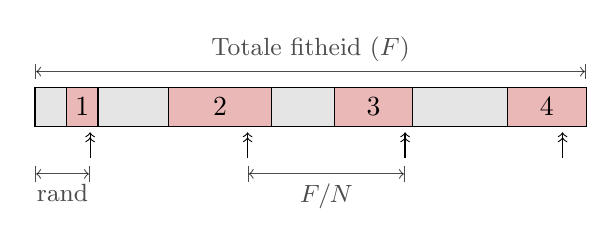
\begin{tikzpicture}

\foreach \x in {0.7,2.7,4.7,6.7}
    \draw[->>] (\x cm,-0.4cm) -- (\x cm,-2pt);

\draw[fill=black,fill opacity=0.1] (0,0) rectangle (7,0.5);

\foreach \x in {0.4,0.8,1.7,3,3.8,4.8,6}
    \draw (\x cm,0pt) -- (\x cm,0.5);

\draw[fill=mymark] (0.4,0) rectangle node {1} (0.8,0.5);
\draw[fill=mymark] (1.7,0) rectangle node {2} (3.0,0.5);
\draw[fill=mymark] (3.8,0) rectangle node {3} (4.8,0.5);
\draw[fill=mymark] (6.0,0) rectangle node {4} (7.0,0.5);

\draw[|<->|,black,opacity=0.7] (0,0.7) -- node[above] {\small Totale fitheid ($F$)} (7,0.7);
\draw[|<->|,black,opacity=0.7] (2.7,-0.6) -- node[below] {\small $F/N$} (4.7,-0.6);
\draw[|<->|,black,opacity=0.7] (0,-0.6) -- node[below] {\small rand} (0.7,-0.6);

%node[anchor=north] {\x};
\end{tikzpicture}
\caption{Visualisatie Stochastic Universal Sampling}
\label{fig:SUS}
\end{figure}
\end{center}


\subsubsection{Algoritme}
Het algoritme die het voorgaande idee implementeert heeft volgende vorm:
	\begin{algorithm}[H]
	 	\caption{Stochastic Universal Sampeling}
		\begin{algorithmic}
		\Require 
			\State $P$, te grote lijst van individuën 
			\State $N_l$, gewenste aantal individuen
		\Ensure returnt een lijst van gekozen individuen
		\Function{SUS}{$P$,$N_t$}
		\State Q $\gets \emptyset$
		\State total $\gets \sum_{x \in P} f(x)$ 
		\State size $\gets \frac{\text{total}}{N_l}$
		\State offset $\gets$ arbitraire waarde uit $\left\lbrack 0,\text{size} \right\rbrack$
		\State $t \gets$ offset
		\For{\textbf{each} $p \in P$} 
		\State $t = t-p.$fitness
		\If{$t<0$}
			\State $Q = Q \cup \lbrace p \rbrace$
			\State $t = t+$offset
		\EndIf
		\EndFor		
		\State \Return i
		\EndFunction

		
		\end{algorithmic}
		\label{alg:SUS}
	\end{algorithm}		
% subsubsection  (end)

\subsubsection{Complexiteit}
\label{ssub:SUSComplexity}
We moeten nagenoeg alle individuen in de populatie overopen. We kunnen dus stellen dat de complexiteit $ \Theta(\abs{P})$ is, met $\abs{P}$ de grootte van de populatie. Nu is $\abs{P}$ geen argument van ons programma. Dus bekomen we een complexiteit van \[T(n) = \Theta(1)\]
% subsubsection  (end)

%\section{Bronnen}
Er moet vermeld worden dat het icosagon bestand afkomstig is van Jonathan Peck. 

\end{document}
%\documentclass[11pt,a4paper]{article}
\usepackage[utf8]{inputenc}
\usepackage[dutch]{babel}
\usepackage{pgfplots}
\usepgfplotslibrary{units}
\usepackage{float}
\usepackage{amsmath,amsthm}
\usepackage{amsfonts}
\usepackage{amssymb,marvosym}
\usepackage[left=2cm,right=2cm,top=2.5cm,bottom=2cm]{geometry}
\usepackage{graphicx}
\usepackage{multicol}
\usepackage{enumerate}
\usepackage{fancyhdr}
\pagestyle{fancy}
\usepackage{algorithm}
\usepackage{algpseudocode}
\usepackage{pgfplots}
\usepackage{multirow}
\usepackage{tikz}
\usetikzlibrary{arrows}
\usetikzlibrary{calc}

\floatname{algorithm}{Algoritme}


\usepackage[font=small,labelfont=bf]{caption}
\captionsetup[table]{aboveskip=-0.8em}
\captionsetup[table]{belowskip=-0.7pt}


\lhead {Proj. DAII: Genetische algoritmen} 
\chead{BAZ(~ \thepage ~ )NGA} 
\rhead{Robbert Gurdeep Singh}


\cfoot{} % get rid of the page number 

\usepackage{hyperref}
\usepackage{chngcntr}
\counterwithin*{section}{part}
\counterwithin{algorithm}{section}
\counterwithin{table}{section}
\counterwithin{figure}{section}

\hypersetup{
    colorlinks=false,
    pdfborder={0 0 0},
}

\author{Robbert Gurdeep Singh}
\title{{Project Algoritmen en datastructuren III}\\ \Huge Gedistribueerde Genetische algoritmen}
%\date{}



\pgfplotsset{compat=1.8}


\newcommand{\drawGraph}[4]{
\begin{tikzpicture}
\begin{axis}[scale only axis, 
	%x-as	
    xmin=0,
	xlabel=#1,	
	%y-as
	ylabel=#2,
	ymin=0,
	%Style
	height=5em,width=.37\textwidth,
	enlargelimits=0.05,
	grid=major,	legend pos=south east
]
#3
\end{axis}
\end{tikzpicture}
}


\newcommand{\lxaxis}[3]{\begin{tikzpicture}
\begin{axis}[scale only axis, 
cycle list name=exotic,
    xmode=log,
    log ticks with fixed point,
	%x-as	
	xlabel=#2,	
	%y-as
	ylabel=#1,
	ymin=0,
	%Style
	height=5em,width=.37\textwidth,
	enlargelimits=0.05,
	grid=major,	legend pos=south east
]
#3

\end{axis}
\end{tikzpicture}}

\newcommand{\rlxaxis}[3]{\begin{tikzpicture}
\begin{axis}[scale only axis, 
cycle list name=exotic,
    xmode=log,
    log ticks with fixed point,
	%x-as	
	xlabel=#2,	
	%y-as
	ylabel=#1,
	%Style
	height=5em,width=.37\textwidth,
	enlargelimits=0.05,
	grid=major,	legend pos=south east
]
#3

\end{axis}
\end{tikzpicture}}

\newcommand{\nxaxis}[3]{\begin{tikzpicture}
\begin{axis}[scale only axis,
cycle list name=exotic, 
	%x-as	
    xmin=0,
	xlabel=#2,	
	%y-as
	ylabel=#1,
	ymin=0,
	%Style
	height=5em,width=.37\textwidth,
	enlargelimits=0.05,
	grid=major,	legend pos=south east
]
#3

\end{axis}
\end{tikzpicture}}


\newcommand{\nxaxisr}[3]{\begin{tikzpicture}
\begin{axis}[scale only axis,
cycle list name=exotic, 
	%x-as	
	xlabel=#2,	
	%y-as
	ylabel=#1,
	ymin=0,
	%Style
	height=5em,width=.37\textwidth,
	enlargelimits=0.05,
	grid=major,	legend pos=south east
]
#3

\end{axis}
\end{tikzpicture}}

\newcommand{\rnxaxis}[3]{\begin{tikzpicture}
\begin{axis}[scale only axis, 
cycle list name=exotic,
	%x-as	
    xmin=0,
	xlabel=#2,	
	%y-as
	ylabel=#1,
	%Style
	height=5em,width=.37\textwidth,
	enlargelimits=0.05,
	grid=major,	legend pos=south east
]
#3

\end{axis}
\end{tikzpicture}}


\newcommand{\rnxaxisr}[3]{\begin{tikzpicture}
\begin{axis}[scale only axis, 
cycle list name=exotic,
	%x-as	
	xlabel=#2,	
	%y-as
	ylabel=#1,
	%Style
	height=5em,width=.37\textwidth,
	enlargelimits=0.05,
	grid=major,	legend pos=south east
]
#3

\end{axis}
\end{tikzpicture}}


\newcommand{\itemMB}[1]{
	\item[$\boldsymbol{#1}$:]
}

\newcommand{\itembf}[1]{
	\item \textbf{#1}:
}



\newcommand{\abs}[1]{
	\lvert #1 \rvert
}

\newcommand{\addploti}[1]{\addplot table [y=i, x=testValue, col sep=comma] {../../tests/param_results/#1.log};}
\newcommand{\addplotf}[1]{\addplot table [y=f, x=testValue, col sep=comma] {../../tests/param_results/#1.log};}
\newcommand{\addplott}[1]{\addplot table [y=t, x=testValue, col sep=comma] {../../tests/param_results/#1.log};}

\definecolor{mymark}{HTML}{EBB8B8}

\begin{document}

\twocolumn[\begin{@twocolumnfalse}
    \maketitle
    
    \begin{abstract}
    	{\em
    	In dit verslag bespreken we de implementatie van een genetisch algoritmen. We onderzoeken wat de optimale parameters zijn en vergelijken enkele algoritmen.
    	}
    \end{abstract}
    
\end{@twocolumnfalse}]
\subsection{Mutation}
\label{sub:Mutation}
We willen er voor zorgend dat de diversiteit in de samenleving niet verdwijnt. Daarom zullen we kleine afwijkingen introduceren.

\subsubsection{Idee}
Nadat er een kind gevormd is zullen we het met een bepaalde kans laten veranderen. Dat is dus dat er 1 punt lichtjes wordt verplaatst. Deze verplaatsing doen we door een nieuw punt te kiezen in de omgeving van het oorspronkelijk punt. Als dit gerandomiseerd punt buiten de figuur valt, proberen we het opnieuw met een kleinere omgeving.

\subsubsection{Algoritme}
\label{ssub:MutationAlgorithm}
Het algoritme die het voorgaande idee implementeert heeft volgende vorm:
	\begin{algorithm}[H]
	 	\caption{Mutatie}
		\begin{algorithmic}
		\Require \State $I$, een individu \State $poly$ de veelhoek
		\Ensure $I$ is mischien gemuteeerd 
		
		\If{\texttt{rand() \% MUTATION\_1\_IN} = 0}
			\State $P \gets$ arbitrair punt van $I$ 
			\State $r \gets$ diameter van poly / \texttt{MUTATION\_DELTA}
			\Repeat 
			\State kies $(x_{new},y_{new}) \in \mathring{B}(P,r)$
			\State $r \gets r/2$
			\Until{$(x_{new},y_{new}) \in poly$}
		\EndIf		
		\end{algorithmic}
		\label{alg:Mutation}
	\end{algorithm}		
% subsubsection  (end)
Hierbij is de ``diameter van poly'' de maximale afstand tussen 2 punten van de convexe veelhoek.

\subsubsection{Implementatie}
\label{ssub:MutationImplementation}
De diagonaal die we in sectie \ref{ssub:MutationAlgorithm} beschouwen, word bij de implementatie zeer ruw benaderd door de diagonaal van het omgestoten vierkant te bepalen.

De implementatie is terug te vinden in \\
\texttt{do\_mutation()} van \texttt{genetic\_base.c}
% subsubsection  (end)

\subsubsection{Complexiteit}
\label{ssub:MutationComplexity}
Het kiezen van een nieuw punt is een operatie die in constante tijd kan gebeuren. Het nagaan dat het in de figuur ligt vraagt echter $\Theta(z)$ met $z$ het aantal zijden in de veelhoek\footnote{Zie Subsectie \ref{sub:algo-pt-in-poly}}.
% subsubsection  (end)

%\section{Bronnen}
Er moet vermeld worden dat het icosagon bestand afkomstig is van Jonathan Peck. 

\end{document}
%\documentclass[11pt,a4paper]{article}
\usepackage[utf8]{inputenc}
\usepackage[dutch]{babel}
\usepackage{pgfplots}
\usepgfplotslibrary{units}
\usepackage{float}
\usepackage{amsmath,amsthm}
\usepackage{amsfonts}
\usepackage{amssymb,marvosym}
\usepackage[left=2cm,right=2cm,top=2.5cm,bottom=2cm]{geometry}
\usepackage{graphicx}
\usepackage{multicol}
\usepackage{enumerate}
\usepackage{fancyhdr}
\pagestyle{fancy}
\usepackage{algorithm}
\usepackage{algpseudocode}
\usepackage{pgfplots}
\usepackage{multirow}
\usepackage{tikz}
\usetikzlibrary{arrows}
\usetikzlibrary{calc}

\floatname{algorithm}{Algoritme}


\usepackage[font=small,labelfont=bf]{caption}
\captionsetup[table]{aboveskip=-0.8em}
\captionsetup[table]{belowskip=-0.7pt}


\lhead {Proj. DAII: Genetische algoritmen} 
\chead{BAZ(~ \thepage ~ )NGA} 
\rhead{Robbert Gurdeep Singh}


\cfoot{} % get rid of the page number 

\usepackage{hyperref}
\usepackage{chngcntr}
\counterwithin*{section}{part}
\counterwithin{algorithm}{section}
\counterwithin{table}{section}
\counterwithin{figure}{section}

\hypersetup{
    colorlinks=false,
    pdfborder={0 0 0},
}

\author{Robbert Gurdeep Singh}
\title{{Project Algoritmen en datastructuren III}\\ \Huge Gedistribueerde Genetische algoritmen}
%\date{}



\pgfplotsset{compat=1.8}


\newcommand{\drawGraph}[4]{
\begin{tikzpicture}
\begin{axis}[scale only axis, 
	%x-as	
    xmin=0,
	xlabel=#1,	
	%y-as
	ylabel=#2,
	ymin=0,
	%Style
	height=5em,width=.37\textwidth,
	enlargelimits=0.05,
	grid=major,	legend pos=south east
]
#3
\end{axis}
\end{tikzpicture}
}


\newcommand{\lxaxis}[3]{\begin{tikzpicture}
\begin{axis}[scale only axis, 
cycle list name=exotic,
    xmode=log,
    log ticks with fixed point,
	%x-as	
	xlabel=#2,	
	%y-as
	ylabel=#1,
	ymin=0,
	%Style
	height=5em,width=.37\textwidth,
	enlargelimits=0.05,
	grid=major,	legend pos=south east
]
#3

\end{axis}
\end{tikzpicture}}

\newcommand{\rlxaxis}[3]{\begin{tikzpicture}
\begin{axis}[scale only axis, 
cycle list name=exotic,
    xmode=log,
    log ticks with fixed point,
	%x-as	
	xlabel=#2,	
	%y-as
	ylabel=#1,
	%Style
	height=5em,width=.37\textwidth,
	enlargelimits=0.05,
	grid=major,	legend pos=south east
]
#3

\end{axis}
\end{tikzpicture}}

\newcommand{\nxaxis}[3]{\begin{tikzpicture}
\begin{axis}[scale only axis,
cycle list name=exotic, 
	%x-as	
    xmin=0,
	xlabel=#2,	
	%y-as
	ylabel=#1,
	ymin=0,
	%Style
	height=5em,width=.37\textwidth,
	enlargelimits=0.05,
	grid=major,	legend pos=south east
]
#3

\end{axis}
\end{tikzpicture}}


\newcommand{\nxaxisr}[3]{\begin{tikzpicture}
\begin{axis}[scale only axis,
cycle list name=exotic, 
	%x-as	
	xlabel=#2,	
	%y-as
	ylabel=#1,
	ymin=0,
	%Style
	height=5em,width=.37\textwidth,
	enlargelimits=0.05,
	grid=major,	legend pos=south east
]
#3

\end{axis}
\end{tikzpicture}}

\newcommand{\rnxaxis}[3]{\begin{tikzpicture}
\begin{axis}[scale only axis, 
cycle list name=exotic,
	%x-as	
    xmin=0,
	xlabel=#2,	
	%y-as
	ylabel=#1,
	%Style
	height=5em,width=.37\textwidth,
	enlargelimits=0.05,
	grid=major,	legend pos=south east
]
#3

\end{axis}
\end{tikzpicture}}


\newcommand{\rnxaxisr}[3]{\begin{tikzpicture}
\begin{axis}[scale only axis, 
cycle list name=exotic,
	%x-as	
	xlabel=#2,	
	%y-as
	ylabel=#1,
	%Style
	height=5em,width=.37\textwidth,
	enlargelimits=0.05,
	grid=major,	legend pos=south east
]
#3

\end{axis}
\end{tikzpicture}}


\newcommand{\itemMB}[1]{
	\item[$\boldsymbol{#1}$:]
}

\newcommand{\itembf}[1]{
	\item \textbf{#1}:
}



\newcommand{\abs}[1]{
	\lvert #1 \rvert
}

\newcommand{\addploti}[1]{\addplot table [y=i, x=testValue, col sep=comma] {../../tests/param_results/#1.log};}
\newcommand{\addplotf}[1]{\addplot table [y=f, x=testValue, col sep=comma] {../../tests/param_results/#1.log};}
\newcommand{\addplott}[1]{\addplot table [y=t, x=testValue, col sep=comma] {../../tests/param_results/#1.log};}

\definecolor{mymark}{HTML}{EBB8B8}

\begin{document}

\twocolumn[\begin{@twocolumnfalse}
    \maketitle
    
    \begin{abstract}
    	{\em
    	In dit verslag bespreken we de implementatie van een genetisch algoritmen. We onderzoeken wat de optimale parameters zijn en vergelijken enkele algoritmen.
    	}
    \end{abstract}
    
\end{@twocolumnfalse}]
\subsection{Crossover}
\label{sub:crossover}
Als 2 individuen geselecteerd zijn om te paren, dan moeten wij daaruit een kind creeren dat eigenscchappen van beide ouders bevat. 
Alternatief kunnen we er ook voor kiezen om een willikeurig aantal keer te wisslen.
\subsubsection{Algoritme}
	\begin{algorithm}[H]
	 	\caption{1-point Crossover}
		\begin{algorithmic}
		\Require $mama, papa$ de ouders
		\Ensure $kind$ is een nieuw kind dat genetisch gelijkend is met de ouders
		
		\State $n \gets $ aantal punten in $mama$
		\State $r \gets$ arbitrair getal in $\lbrace 1, \dots , n-2\rbrace$
		\For{i \textbf{from} 0 \textbf{to} $r$}
			\State $kind$.punten[$i$] $\gets mama$.punten[$i$]
		\EndFor
		\For{i \textbf{from} $r+1$ \textbf{to} $n-1$}
			\State $kind$.punten[$i$] $\gets papa$.punten[$i$]
		\EndFor
		\end{algorithmic}
		\label{alg:crossover-1point}
	\end{algorithm}		

	\begin{algorithm}[H]
	 	\caption{random Crossover}
		\begin{algorithmic}
		\Require $mama, papa$ de ouders
		\Ensure $kind$ is een nieuw kind dat genetisch gelijkend is met de ouders
		
		\State $n \gets $ aantal punten in $mama$
		\State $r \gets$ arbitrair getal in $\lbrace 1, \dots , n-2\rbrace$
		\For{i \textbf{from} 0 \textbf{to} $n-1$}
		\State $oud$ $\gets$ arbitrare waarde uit $\lbrace mama, papa \rbrace$
		\State $kind$.punten[$i$] $\gets oud$.punten[$i$]
			
		\EndFor

		\end{algorithmic}
		\label{alg:crossover-random}
	\end{algorithm}		



\subsubsection{Complexiteit}
\label{sub:alg_crossover_compl}
Een crossover kopieert $n$ waarden. Het is dus $T(n)=\Theta(n)$


% subsection  (end)


\subsubsection{Implementatie}
Het bestand \texttt{genetic\_base.c} bevat de implementatie van Algoritme \ref{alg:crossover-1point} en \ref{alg:crossover-random} in de functie 
\\ \texttt{do\_crossover()}. 
Het bestand bevat beide implementaties, bij compilatie kan er tussen beide gekozen worden door we waarde van \\ \texttt{RANDOM\_CROSSOVER} in te stellen met de \texttt{-D} vlag. Standaard staat deze waarde ingesteld op 1-point, de reden hiervoor vind u in sectie \ref{ssub:crossover_type}.


%\section{Bronnen}
Er moet vermeld worden dat het icosagon bestand afkomstig is van Jonathan Peck. 

\end{document}

%\documentclass[11pt,a4paper]{article}
\usepackage[utf8]{inputenc}
\usepackage[dutch]{babel}
\usepackage{pgfplots}
\usepgfplotslibrary{units}
\usepackage{float}
\usepackage{amsmath,amsthm}
\usepackage{amsfonts}
\usepackage{amssymb,marvosym}
\usepackage[left=2cm,right=2cm,top=2.5cm,bottom=2cm]{geometry}
\usepackage{graphicx}
\usepackage{multicol}
\usepackage{enumerate}
\usepackage{fancyhdr}
\pagestyle{fancy}
\usepackage{algorithm}
\usepackage{algpseudocode}
\usepackage{pgfplots}
\usepackage{multirow}
\usepackage{tikz}
\usetikzlibrary{arrows}
\usetikzlibrary{calc}

\floatname{algorithm}{Algoritme}


\usepackage[font=small,labelfont=bf]{caption}
\captionsetup[table]{aboveskip=-0.8em}
\captionsetup[table]{belowskip=-0.7pt}


\lhead {Proj. DAII: Genetische algoritmen} 
\chead{BAZ(~ \thepage ~ )NGA} 
\rhead{Robbert Gurdeep Singh}


\cfoot{} % get rid of the page number 

\usepackage{hyperref}
\usepackage{chngcntr}
\counterwithin*{section}{part}
\counterwithin{algorithm}{section}
\counterwithin{table}{section}
\counterwithin{figure}{section}

\hypersetup{
    colorlinks=false,
    pdfborder={0 0 0},
}

\author{Robbert Gurdeep Singh}
\title{{Project Algoritmen en datastructuren III}\\ \Huge Gedistribueerde Genetische algoritmen}
%\date{}



\pgfplotsset{compat=1.8}


\newcommand{\drawGraph}[4]{
\begin{tikzpicture}
\begin{axis}[scale only axis, 
	%x-as	
    xmin=0,
	xlabel=#1,	
	%y-as
	ylabel=#2,
	ymin=0,
	%Style
	height=5em,width=.37\textwidth,
	enlargelimits=0.05,
	grid=major,	legend pos=south east
]
#3
\end{axis}
\end{tikzpicture}
}


\newcommand{\lxaxis}[3]{\begin{tikzpicture}
\begin{axis}[scale only axis, 
cycle list name=exotic,
    xmode=log,
    log ticks with fixed point,
	%x-as	
	xlabel=#2,	
	%y-as
	ylabel=#1,
	ymin=0,
	%Style
	height=5em,width=.37\textwidth,
	enlargelimits=0.05,
	grid=major,	legend pos=south east
]
#3

\end{axis}
\end{tikzpicture}}

\newcommand{\rlxaxis}[3]{\begin{tikzpicture}
\begin{axis}[scale only axis, 
cycle list name=exotic,
    xmode=log,
    log ticks with fixed point,
	%x-as	
	xlabel=#2,	
	%y-as
	ylabel=#1,
	%Style
	height=5em,width=.37\textwidth,
	enlargelimits=0.05,
	grid=major,	legend pos=south east
]
#3

\end{axis}
\end{tikzpicture}}

\newcommand{\nxaxis}[3]{\begin{tikzpicture}
\begin{axis}[scale only axis,
cycle list name=exotic, 
	%x-as	
    xmin=0,
	xlabel=#2,	
	%y-as
	ylabel=#1,
	ymin=0,
	%Style
	height=5em,width=.37\textwidth,
	enlargelimits=0.05,
	grid=major,	legend pos=south east
]
#3

\end{axis}
\end{tikzpicture}}


\newcommand{\nxaxisr}[3]{\begin{tikzpicture}
\begin{axis}[scale only axis,
cycle list name=exotic, 
	%x-as	
	xlabel=#2,	
	%y-as
	ylabel=#1,
	ymin=0,
	%Style
	height=5em,width=.37\textwidth,
	enlargelimits=0.05,
	grid=major,	legend pos=south east
]
#3

\end{axis}
\end{tikzpicture}}

\newcommand{\rnxaxis}[3]{\begin{tikzpicture}
\begin{axis}[scale only axis, 
cycle list name=exotic,
	%x-as	
    xmin=0,
	xlabel=#2,	
	%y-as
	ylabel=#1,
	%Style
	height=5em,width=.37\textwidth,
	enlargelimits=0.05,
	grid=major,	legend pos=south east
]
#3

\end{axis}
\end{tikzpicture}}


\newcommand{\rnxaxisr}[3]{\begin{tikzpicture}
\begin{axis}[scale only axis, 
cycle list name=exotic,
	%x-as	
	xlabel=#2,	
	%y-as
	ylabel=#1,
	%Style
	height=5em,width=.37\textwidth,
	enlargelimits=0.05,
	grid=major,	legend pos=south east
]
#3

\end{axis}
\end{tikzpicture}}


\newcommand{\itemMB}[1]{
	\item[$\boldsymbol{#1}$:]
}

\newcommand{\itembf}[1]{
	\item \textbf{#1}:
}



\newcommand{\abs}[1]{
	\lvert #1 \rvert
}

\newcommand{\addploti}[1]{\addplot table [y=i, x=testValue, col sep=comma] {../../tests/param_results/#1.log};}
\newcommand{\addplotf}[1]{\addplot table [y=f, x=testValue, col sep=comma] {../../tests/param_results/#1.log};}
\newcommand{\addplott}[1]{\addplot table [y=t, x=testValue, col sep=comma] {../../tests/param_results/#1.log};}

\definecolor{mymark}{HTML}{EBB8B8}

\begin{document}

\twocolumn[\begin{@twocolumnfalse}
    \maketitle
    
    \begin{abstract}
    	{\em
    	In dit verslag bespreken we de implementatie van een genetisch algoritmen. We onderzoeken wat de optimale parameters zijn en vergelijken enkele algoritmen.
    	}
    \end{abstract}
    
\end{@twocolumnfalse}]
\section{Keuzes alogoritmen}
Tijdens het optimaliseren van ons project hebben we hier en daar verschillende algoritmen uitgeprobeert om te zien welk resultaat ze opleveren. Hierna bespreken we welke dat zijn en welke we gekozen hebben.
\subsection{Selectie methode geliefden}
\label{sub:algLoverSelection}


\begin{figure}[H]
\nxaxis{Fitness}{Aantal punten}{
	\addplotf{SUS_1_vierkant};
	\addplotf{SUS_0_vierkant};
}
\nxaxis{Iteraties}{Aantal punten}{
	\addploti{SUS_1_icosagon};
	\addploti{SUS_0_icosagon};
}
\nxaxis{Tijd}{Aantal punten}{
	\addplott{SUS_1_vierkant};
	\addplott{SUS_0_vierkant};
}
\caption{Vergelijking van Stochastic Universal Sampling (blauw) en Tournament Selection (oranje) voor selectie van individu's om voort te planten bij het plaatsen van een variabel aantal punten in \texttt{vierkant}.}
\label{graf:algLoverSelection}
\end{figure}
Kijken we naar de grafieken in figuur \ref{graf:algLoverSelection} dan zien we dat Stochastic Universal Sampeling steeds een factor slechter trager is terwijl het resultaat even goed is. We merken ook dat het tijdsverschil komt door het hoger aantal iteraties bij Sotochastic Universal Selection. Met andere woorden, hier hebben we getoond dat Tournament de betere keuze is in tegenstelling tot wat enkele bronnen ons trachten te doen geloven. Dit kan uiteraard liggen aan het soort probleem.

% subsection  (end)

\subsection{Crossover}
We hebben nog niet genoeg seks gehad om dit te weten. (Lees: we hebben nog geen resultaten voor deze test, but hey we're woring on it)

Maar hypothetisch gezien moet ons random algoritme slechter scoren, hier volgt mijn brainfart over hoe het in elkaar steekt.
%todo

We (zouden) zien dat het algoritme met random wijzigingen slechter presteert zowel in uitvoeringstijd als in kwaliteit.

Dit is te verwachten omdat de fitheid afhangt van de onderlinge ligging van de punten. Als de punten random worden gekozen in de kinderen, verlies je de samenhang die er reeds bestond. Waardoor de fitheid over het algemeen slechter zal zijn dan bij 1-point crossover.

\section{Parameter Optimalisatie}
\subsection{Aantal individuen}
Een eerste parameter die we zullen onderzoeken is \texttt{NUM\_INDIVIDUS}. Deze parameter stelt het aantal individuen in de populatie voor. In dit verslag wordt deze waarde ook $N_p$ genoemd.
\begin{figure}[H]
\rlxaxis{Fitness}{Aantal individus}{
	\addplotf{NUM_INDIVIDUS_vierkant_15};
}
\lxaxis{Iteraties}{Aantal individus}{
	\addploti{NUM_INDIVIDUS_vierkant_15};
}
\lxaxis{Tijd}{Aantal individus}{
	\addplott{NUM_INDIVIDUS_vierkant_15};
}



  \caption{Correlatie tussen het aantal individuen op convergentie snelheid en kwaliteit. Reslutaten voor het plaatsen van 15 punten in \texttt{vierkant.poly}.}
  \label{graf:numIndividus}
\end{figure}
Kijken ze naar de grafieken uit figuur \ref{graf:numIndividus}, dan zien we dat het fitheid stijgt naarmate het het aantal individuen stijgt. Initieel is er een sterke stijging die afvlakt naarmate we honderd individuen bereiken. Helaas groeit de uitvoertijd ook lineair\footnote{Merk de logaritmische schaal van de $x$-as op.} met het aantal individuen. We kiezen voor een populatie van \textbf{100~individuen}. 
% subsection  (end)
%
%
%
%
%
\subsection{Hoeveelheid seks}
Nu onderzoeken we de invloed van \texttt{LOVER\_PERCENT}. Deze parameter geeft aan welk percentage van de populatie zich voortplant per iteratie.
\begin{figure}[H]
\rnxaxis{Fitness}{Sekspercentage}{
	\addplotf{LOVER_PERCENT_vierkant_15};
	\addplotf{LOVER_PERCENT_soos_15};
}
\nxaxis{Iteraties}{Sekspercenntage}{
	\addploti{LOVER_PERCENT_vierkant_15};
	\addploti{LOVER_PERCENT_soos_15}; 
}
\nxaxis{Tijd (s)}{Sekspercentage}{
	\addplott{LOVER_PERCENT_vierkant_15};
	\addplott{LOVER_PERCENT_soos_15};
}



\caption{Correlatie tussen de hoeveelheid seks en de convergentie snelheid en kwaliteit. Reslutaten voor het plaatsen van 15 punten in \texttt{vierkant.poly} (blauw) en \texttt{soos.poly} (oranje).}
\label{graf:numLovers}
\end{figure}
In de eerste grafiek van figuur \ref{graf:numLovers} zien we dat de aanwezigheid van seks noodzakelijk is voor het behalen van een optimale fitheid. Daarnaast zien we dat het niet echt uit maakt hoeveel seks er is, als het er maar is. De stijging vlakt snel af, na 5\% is de stijging nog maar miniem. De andere grafieken uit dezelfde figuur tonen ons dat hoe meer seks er is hoe langer het duurt om te convergeren. We kiezen ervoor om tijdens elke iteratie \textbf{30\%} van de populatie seks te laten hebben. Merk op dat we niet 5\% kiezen hoewel de grafiek dit suggereert. Als we de data grondiger bestuderen zien we dat de waarde van de fitheid monotoon blijft stijgen. We kiezen er voor om een wat tijd en ruimte op te offeren voor een iets beter resultaat.

 % subsection  (end)



\subsection{Hoeveelheid mutatie}
Als kinderen geboren worden krijgen ze door ons genetisch algoritme een mutatie. Het is duidelijk dat de grootte van deze mutatie aangepast moet zijn aan de grootte van de figuur. Daarom kiezen we telkens een punt in een cirkel die als diameter een fractie van de diameter van de figuur heeft. Deze fractie wordt voorgesteld door de parameter \texttt{MUTATION\_DELTA}.
\begin{figure}[H]
\rlxaxis{Fitness}{\texttt{MUTATION\_DELTA}}{
	\addplotf{MUTATION_DELTA_vierkant_15};
}
\rlxaxis{Fitness}{\texttt{MUTATION\_DELTA}}{
	\addplotf{MUTATION_DELTA_soos_15};
}
\rlxaxis{Fitness}{\texttt{MUTATION\_DELTA}}{
	\addplotf{MUTATION_DELTA_icosagon_15};
}
\caption{Corelatie \texttt{MUTATION\_DELTA} en de bekomen fitheid voor het plaatsen van 15 punten in \texttt{vierkant}, \texttt{soos} en \texttt{icosagon} (van boven naar onder)}

\label{graf:mutationDeltaFig}
\end{figure}
\begin{figure}[H]
\rnxaxis{Tijd (s)}{\texttt{MUTATION\_DELTA}}{
	\addplott{MUTATION_DELTA_vierkant_15};
}

\caption{Corelatie \texttt{MUTATION\_DELTA} en uitvoertijd voor 15 punten in \texttt{vierkant.poly}}
\label{graf:mutationDeltaTime}
\end{figure}
In de grafieken van figuur~\ref{graf:mutationDeltaFig} zien we dat er telkens een waarde is voor \texttt{MUTATION\_DELTA} die de fitheid optimaliseerd. Helaas zien we ook dat deze sterk afhankelijk is van de figuur. Na veel testen kunnen we besluiten dat de waarde tussen 10 en 100 moet liggen.

We merken op dat als \texttt{MUTATION\_DELTA} te groot is, dat betekend dus heel kleine stappen, de punten zich trager verplaatsen. Waardoor ze trager tot een optimum komen. Deze observatie zien we gereflecteerd in figuur \ref{graf:mutationDeltaTime}.

We kiezen de waarde \texttt{MUTATION\_DELTA = 20}. Dit wil zeggen dat het nieuwe punt zal gekozen worden in een cirkel met diameter die een twintigste is van de totale diameter.

% subsection  (end)
















\subsection{Mutatie kans}
Niet alle kinderen worden gemuteerd. De kans dat een kind muteert wordt voorgesteld door de parameter \texttt{MUTATION\_1\_IN}. De waarde van deze parameter geeft aan per hoeveel beschouwde kinderen er gemiddeld één muteert. 
\begin{figure}[H]
\rlxaxis{Fitness}{Kans (1 op ...)}{
	\addplotf{MUTATION_1_IN_vierkant_15};
	\addplotf{MUTATION_1_IN_soos_15};
}
\lxaxis{Iteraties}{Kans (1 op ...)}{
	\addploti{MUTATION_1_IN_vierkant_15};
	\addploti{MUTATION_1_IN_soos_15};
}
\lxaxis{Tijd (s)}{Kans (1 op ...)}{
	\addplott{MUTATION_1_IN_vierkant_15};
	\addplott{MUTATION_1_IN_soos_15};
}

\caption{Corelatie mutatiekans en de bekomen fitheid voor het plaatsen van 15 punten in \texttt{vierkant} (blauw) en \texttt{soos} (oranje)}

\label{graf:mutation1In}
\end{figure}
De grafieken in Fig. \ref{graf:mutation1In} tonen ons dat hoe kleiner de kans om te muteren is, hoe slechter de fitheid. Om de fitheid te optimaiseren kiezen we dus best een grote kans. We kiezen: \textbf{1 mutatie per 3 kinderen}.



\subsection{Selectie druk}
De selectie druk is een maat voor de waarschijnlijkheid dat enkel de beste individuen zich kunnen voortplanten en lang kunnen leven. In ons programma is deze waarde voorgesteld door de parameter \texttt{SELECTION\_PRESSURE}. Deze parameter wordt gebruikt om de toernooigroote te bepalen bij tournament selection\footnote{Zie sectie \ref{sub:tournament}}.
\begin{figure}[H]
\lxaxis{Fitness}{Toernooigrootte}{
	\addplotf{SELECTION_PRESSURE_vierkant_15};
	\addplotf{SELECTION_PRESSURE_soos_15};
}
\lxaxis{Iteraties}{Toernooigrootte}{
	\addploti{SELECTION_PRESSURE_vierkant_15};
	\addploti{SELECTION_PRESSURE_soos_15};
}
\lxaxis{Tijd}{Toernooigrootte}{
	\addplott{SELECTION_PRESSURE_vierkant_15};
	\addplott{SELECTION_PRESSURE_soos_15};
}


\caption{Inpact van de selectiedruk op de convergentie snelheid en kwaliteit voor het plaatsen van 15 punten in \texttt{vierkant} en \texttt{soos}}
\label{graf:selectionPressure}
\end{figure}
Kijken we naar de grafieken in figuur \ref{graf:selectionPressure}, dan zien we dat de bekomen fitheid nagenoeg constant blijft ongeacht de selectiedruk. Wat wel sterk beïnvloed wordt door de selectie druk is de uitvoertijd en het aantal iteraties. We zien dat de uitvoertijd stijgt als de druk te hoog wordt. Hiervoor kunnen we tweee verkklaringen geven. \begin{itemize}\item de uitvoertijd ligt hoger omdat de toernooien langer duren \item en de uitvoertijd ligt hoger odat enkel de besten gekozen worden waardoor de genetsche diversiteit vernietigd wordt en er dus enkel met mutaties tot een goede oplossing moet worden gekomen.\end{itemize}

Wij hebben gekozen voor een selectiedruk van 5. Wat wil zeggen dat de toernooigrootte 5\% is van de populatiegrootte.

% subsection  (end)

\subsection{Weegfactor exponentieel lopend gemidelde}
om te weten of het programma klaar is met optimalisteren, houden we een gewogen exponentieel gemiddelde bij\footnote{zie ook sectie~\ref{sub:stopcond}}. De weegfactor die we kiezen is dus ook een parrameter die wel willen optimaliseren.
\begin{figure}[H]
\rnxaxis{Fitness}{Weegfactor}{
	\addplotf{WEIGHTING_DECREASE_vierkant_15};
}
\nxaxis{Iteraties}{Weegfactor}{
	\addploti{WEIGHTING_DECREASE_vierkant_15};
}
\nxaxis{Tijd}{Weegfactor}{
	\addplott{WEIGHTING_DECREASE_vierkant_15};
}
\caption{Correlatie weegfactor en convergentie snelheid en kwaliteit voor het plaatsen van 15 punten in \texttt{vierkant}}
\label{graf:weightingFactor}
\end{figure}
We zien wat we verwachten te zien. Hoe hoger de weegfactor hoe beter het resultaat maar ook hoe langer het zal duren om tot dat resultaat te komen. 
We kiezen voor een weegfactor van \textbf{0.95} omdat we een optimaal antwoord willen. Merk op dat we niet kiezen voor 100 omdat het algoritme dat niet meer de waarde zou updateën. 
% subsection  (end)

%\section{Bronnen}
Er moet vermeld worden dat het icosagon bestand afkomstig is van Jonathan Peck. 

\end{document}

\section{Toelichting Code}
Life is life, nanananana....
\label{sec:explainationcode}
\subsection{Pointers}
\label{sub:pointer}
We hebben er voor gekozen om een array van individu's te gebruiken in de plaats van een array van pointers. We kiezen er ook voor om zo weinig \texttt{malloc} en \texttt{free} te gebruiken. Dat is dus dat we de bestaande individuen overschrijven in plaats van nieuwe ruimte te alloceren en dan de vorige te verwijderen.
% subsection  (end)
% section explainationcode (end)

\part{Parralelisering}
Nog niet gedaan...

\part{Beschouwing en conclusies}

\section{Bronnen}
Er moet vermeld worden dat het icosagon bestand afkomstig is van Jonathan Peck. 

\end{document}
